\section{mo\-TS$<$ M $>$ Class Template Reference}
\label{classmo_t_s}\index{moTS@{moTS}}
Tabu Search (TS).  


{\tt \#include $<$mo\-TS.h$>$}

Inheritance diagram for mo\-TS$<$ M $>$::\begin{figure}[H]
\begin{center}
\leavevmode
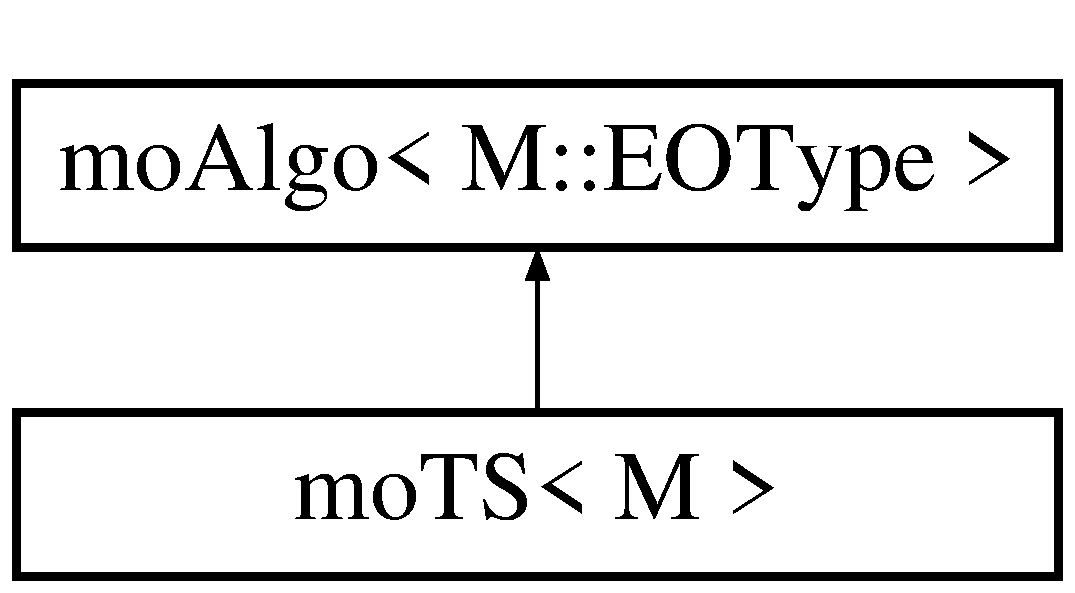
\includegraphics[height=2cm]{classmo_t_s}
\end{center}
\end{figure}
\subsection*{Public Member Functions}
\begin{CompactItemize}
\item 
{\bf mo\-TS} ({\bf mo\-Move\-Init}$<$ M $>$ \&\_\-\_\-move\_\-init, {\bf mo\-Next\-Move}$<$ M $>$ \&\_\-\_\-next\_\-move, {\bf mo\-Move\-Incr\-Eval}$<$ M $>$ \&\_\-\_\-incr\_\-eval, {\bf mo\-Tabu\-List}$<$ M $>$ \&\_\-\_\-tabu\_\-list, {\bf mo\-Aspir\-Crit}$<$ M $>$ \&\_\-\_\-aspir\_\-crit, {\bf mo\-Sol\-Continue}$<$ {\bf EOT} $>$ \&\_\-\_\-cont, eo\-Eval\-Func$<$ {\bf EOT} $>$ \&\_\-\_\-full\_\-eval)
\begin{CompactList}\small\item\em Constructor of a {\bf mo\-TS}{\rm (p.\,\pageref{classmo_t_s})} specifying all the boxes. \item\end{CompactList}\item 
{\bf mo\-TS} ({\bf mo\-Move\-Expl}$<$ M $>$ \&\_\-\_\-move\_\-expl, {\bf mo\-Sol\-Continue}$<$ {\bf EOT} $>$ \&\_\-\_\-cont, eo\-Eval\-Func$<$ {\bf EOT} $>$ \&\_\-\_\-full\_\-eval)
\begin{CompactList}\small\item\em Constructor with less parameters. \item\end{CompactList}\item 
bool {\bf operator()} ({\bf EOT} \&\_\-\_\-sol)
\begin{CompactList}\small\item\em Function which launchs the Tabu Search. \item\end{CompactList}\end{CompactItemize}
\subsection*{Private Types}
\begin{CompactItemize}
\item 
typedef M::EOType {\bf EOT}\label{classmo_t_s_90d19d468c12ab5bd796948ce1ce79b1}

\begin{CompactList}\small\item\em Alias for the type. \item\end{CompactList}\item 
typedef EOT::Fitness {\bf Fitness}\label{classmo_t_s_aa0eefbb17111422e495d1255f876fca}

\begin{CompactList}\small\item\em Alias for the fitness. \item\end{CompactList}\end{CompactItemize}
\subsection*{Private Attributes}
\begin{CompactItemize}
\item 
{\bf mo\-Move\-Expl}$<$ M $>$ \& {\bf move\_\-expl}\label{classmo_t_s_06914ddc90ca96e9158c8dbe182a7865}

\begin{CompactList}\small\item\em Neighborhood explorer. \item\end{CompactList}\item 
{\bf mo\-Sol\-Continue}$<$ {\bf EOT} $>$ \& {\bf cont}\label{classmo_t_s_969371cd2202f3d29cbb426f57ac7d3a}

\begin{CompactList}\small\item\em Stop criterion. \item\end{CompactList}\item 
eo\-Eval\-Func$<$ {\bf EOT} $>$ \& {\bf full\_\-eval}\label{classmo_t_s_fb67eddae5d0bfca4ed881995523231e}

\begin{CompactList}\small\item\em Full evaluation function. \item\end{CompactList}\end{CompactItemize}
\subsection*{Static Private Attributes}
\begin{CompactItemize}
\item 
static bool {\bf first\_\-time} = true\label{classmo_t_s_564bc1969548ccbd9bb7e76f92898de0}

\begin{CompactList}\small\item\em Boolean allowing to initialise the ptread\_\-mutex\_\-t in the constructor. \item\end{CompactList}\item 
static pthread\_\-mutex\_\-t {\bf mutex}\label{classmo_t_s_688f9ba42eb33cae6431f4f4eb65b9e9}

\begin{CompactList}\small\item\em The lock. \item\end{CompactList}\end{CompactItemize}


\subsection{Detailed Description}
\subsubsection*{template$<$class M$>$ class mo\-TS$<$ M $>$}

Tabu Search (TS). 

Generic algorithm that describes a tabu search. 



Definition at line 30 of file mo\-TS.h.

\subsection{Constructor \& Destructor Documentation}
\index{moTS@{mo\-TS}!moTS@{moTS}}
\index{moTS@{moTS}!moTS@{mo\-TS}}
\subsubsection{\setlength{\rightskip}{0pt plus 5cm}template$<$class M$>$ {\bf mo\-TS}$<$ M $>$::{\bf mo\-TS} ({\bf mo\-Move\-Init}$<$ M $>$ \& {\em \_\-\_\-move\_\-init}, {\bf mo\-Next\-Move}$<$ M $>$ \& {\em \_\-\_\-next\_\-move}, {\bf mo\-Move\-Incr\-Eval}$<$ M $>$ \& {\em \_\-\_\-incr\_\-eval}, {\bf mo\-Tabu\-List}$<$ M $>$ \& {\em \_\-\_\-tabu\_\-list}, {\bf mo\-Aspir\-Crit}$<$ M $>$ \& {\em \_\-\_\-aspir\_\-crit}, {\bf mo\-Sol\-Continue}$<$ {\bf EOT} $>$ \& {\em \_\-\_\-cont}, eo\-Eval\-Func$<$ {\bf EOT} $>$ \& {\em \_\-\_\-full\_\-eval})\hspace{0.3cm}{\tt  [inline]}}\label{classmo_t_s_2be23f4524733ee6f37b71310d76407e}


Constructor of a {\bf mo\-TS}{\rm (p.\,\pageref{classmo_t_s})} specifying all the boxes. 

In this constructor, a {\bf mo\-TSMove\-Loop\-Expl}{\rm (p.\,\pageref{classmo_t_s_move_loop_expl})} is instanciated.

\begin{Desc}
\item[Parameters:]
\begin{description}
\item[{\em \_\-\_\-move\_\-init}]move initialisation \item[{\em \_\-\_\-next\_\-move}]neighborhood explorer \item[{\em \_\-\_\-incr\_\-eval}]efficient evaluation \item[{\em \_\-\_\-tabu\_\-list}]tabu list \item[{\em \_\-\_\-aspir\_\-crit}]aspiration criterion \item[{\em \_\-\_\-cont}]stop criterion \item[{\em \_\-\_\-full\_\-eval}]full evaluation function \end{description}
\end{Desc}


Definition at line 59 of file mo\-TS.h.

References mo\-TS$<$ M $>$::first\_\-time, and mo\-TS$<$ M $>$::mutex.\index{moTS@{mo\-TS}!moTS@{moTS}}
\index{moTS@{moTS}!moTS@{mo\-TS}}
\subsubsection{\setlength{\rightskip}{0pt plus 5cm}template$<$class M$>$ {\bf mo\-TS}$<$ M $>$::{\bf mo\-TS} ({\bf mo\-Move\-Expl}$<$ M $>$ \& {\em \_\-\_\-move\_\-expl}, {\bf mo\-Sol\-Continue}$<$ {\bf EOT} $>$ \& {\em \_\-\_\-cont}, eo\-Eval\-Func$<$ {\bf EOT} $>$ \& {\em \_\-\_\-full\_\-eval})\hspace{0.3cm}{\tt  [inline]}}\label{classmo_t_s_508e675c4232cf2ca06dded931c90bab}


Constructor with less parameters. 

The explorer is given in the parameters.

\begin{Desc}
\item[Parameters:]
\begin{description}
\item[{\em \_\-\_\-move\_\-expl}]the explorer (generally different that a {\bf mo\-TSMove\-Loop\-Expl}{\rm (p.\,\pageref{classmo_t_s_move_loop_expl})}) \item[{\em \_\-\_\-cont}]stop criterion \item[{\em \_\-\_\-full\_\-eval}]full evaluation function \end{description}
\end{Desc}


Definition at line 81 of file mo\-TS.h.

References mo\-TS$<$ M $>$::first\_\-time, and mo\-TS$<$ M $>$::mutex.

\subsection{Member Function Documentation}
\index{moTS@{mo\-TS}!operator()@{operator()}}
\index{operator()@{operator()}!moTS@{mo\-TS}}
\subsubsection{\setlength{\rightskip}{0pt plus 5cm}template$<$class M$>$ bool {\bf mo\-TS}$<$ M $>$::operator() ({\bf EOT} \& {\em \_\-\_\-sol})\hspace{0.3cm}{\tt  [inline]}}\label{classmo_t_s_94d25a76fe1bc9ef0bbd0358ff55aceb}


Function which launchs the Tabu Search. 

Algorithm of the tabu search. As a {\bf mo\-SA}{\rm (p.\,\pageref{classmo_s_a})} or a {\bf mo\-HC}{\rm (p.\,\pageref{classmo_h_c})}, it can be used for HYBRIDATION in an evolutionary algorithm. For security a lock (pthread\_\-mutex\_\-t) is closed during the algorithm.

\begin{Desc}
\item[Parameters:]
\begin{description}
\item[{\em \_\-\_\-sol}]a solution to improve. \end{description}
\end{Desc}
\begin{Desc}
\item[Returns:]TRUE. \end{Desc}


Definition at line 104 of file mo\-TS.h.

References mo\-TS$<$ M $>$::full\_\-eval, and mo\-TS$<$ M $>$::mutex.

The documentation for this class was generated from the following file:\begin{CompactItemize}
\item 
mo\-TS.h\end{CompactItemize}
